\documentclass[tikz,border=4pt]{standalone}
\usepackage{fontspec}\usepackage{xcolor}\usetikzlibrary{arrows.meta,calc,positioning}
\setsansfont{Lato}
\begin{document}
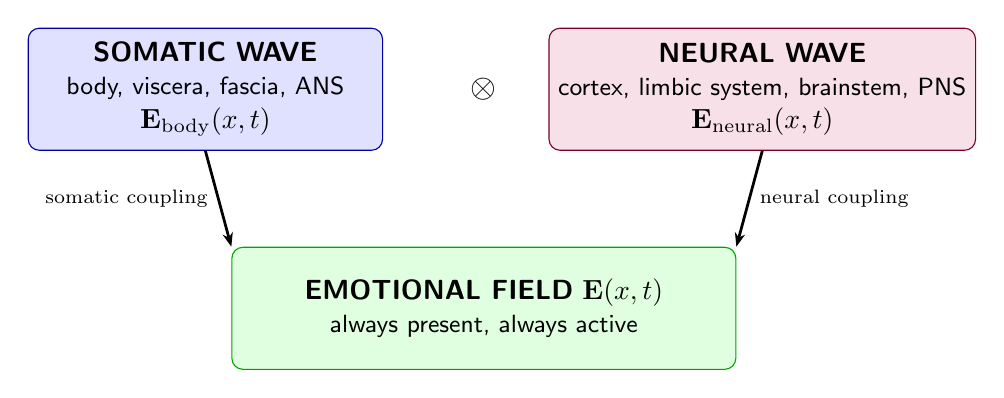
\begin{tikzpicture}[font=\sffamily,box/.style={rounded corners=4pt,draw=#1!65!black,fill=#1!12,minimum width=4.5cm,minimum height=1.55cm,align=center},arrow/.style={-{Stealth[length=5pt]},line width=1pt}]
\node[box=blue] (body) {\textbf{SOMATIC WAVE}\\\small body, viscera, fascia, ANS\\$\mathbf E_{\mathrm{body}}(x,t)$};
\node[box=purple,right=2.1cm of body] (neural) {\textbf{NEURAL WAVE}\\\small cortex, limbic system, brainstem, PNS\\$\mathbf E_{\mathrm{neural}}(x,t)$};
\node[box=green,minimum width=6.4cm,below=2cm of $(body)!0.5!(neural)$] (field) {\textbf{EMOTIONAL FIELD} $\mathbf E(x,t)$\\\small always present, always active};
\draw[arrow] (body.south) -- (field.north west) node[midway,left,font=\scriptsize]{somatic coupling};
\draw[arrow] (neural.south) -- (field.north east) node[midway,right,font=\scriptsize]{neural coupling};
\node[font=\large] at ($(body)!0.5!(neural)$) {$\otimes$};
\end{tikzpicture}\end{document}
